\documentclass{article}

%%%%%%%%%%%%%%%%%%%%%%%%%%%%%%%%%%%%%%%%%%%%%%%%%%%%%%%
%                   Useful packages                   %
%%%%%%%%%%%%%%%%%%%%%%%%%%%%%%%%%%%%%%%%%%%%%%%%%%%%%%%

% I doubt you need more than this. If you are stuck with commands, google is your best friend.

\usepackage[utf8]{inputenc}     % for éô
\usepackage[english]{babel}     % for proper word breaking at line ends
\usepackage[a4paper, left=1.5in, right=1.5in, top=1.5in, bottom=1.5in]{geometry}
                                % for page size and margin settings
\usepackage{graphicx}           % for image pathing
\usepackage{amsmath,amssymb}    % for better equations
\usepackage{amsthm}             % for better theorem styles
\usepackage{mathtools}          % for greek math symbol formatting
\usepackage{enumitem}           % for control of 'enumerate' numbering
\usepackage{listings}           % for control of 'itemize' spacing
\usepackage{hyperref}           % page numbers and '\ref's become clickable
\usepackage{caption}            % for the captions of subfigures
\usepackage{float}              % for the 'H' positioning of figures
\usepackage{subfig}             % for subfigures
\usepackage{bm}                 % for bold math symbols
\usepackage{subfiles}           % for loading in files
\usepackage{listings}           % for the formatting of code blocks
\lstset{                        % for the boxing of code blocks
    basicstyle=\footnotesize, 
    frame=single,
    breaklines=true,
}

\setlength{\parindent}{0cm}     % removes the paragraph indentation

\begin{document}

%%%%%%%%%%%%%%%%%%%%%%%%%%%%%%%%%%%%%%%%%%%%%%%%%%%%%%%
%                      The header                     %
%%%%%%%%%%%%%%%%%%%%%%%%%%%%%%%%%%%%%%%%%%%%%%%%%%%%%%%

\begin{center}
\scshape 
	\large{\textbf{AI PRINCIPLES \& TECHNIQUES}}\\[5mm]
	\large{Assignment Title}\\[5mm]
	\normalsize{NAME LASTNAME \hfill \textit{STUDENT NUMBER}}\\
	\normalsize{NAME LASTNAME \hfill \textit{STUDENT NUMBER}}\\
	\normalsize{Radboud University \hfill \textit{DATE}}	\rule{\textwidth}{0.4pt} \\
	\vspace{0.3\baselineskip}
\end{center}

%%%%%%%%%%%%%%%%%%%%%%%%%%%%%%%%%%%%%%%%%%%%%%%%%%%%%%%
%                   The text contents                 %
%%%%%%%%%%%%%%%%%%%%%%%%%%%%%%%%%%%%%%%%%%%%%%%%%%%%%%%

\section{Introduction}
This document contains the packages needed to create the example report for the assignments in Overleaf. If you already are familiar with Overleaf and Latex feel free to just delete the text contents section. For people less familiar with Overleaf or Latex this document shows some basic commands to create a report such as the one given as an example. Please use the source side of this document to navigate it properly.\\

In Overleaf we can use a double backward slash to print a blank line. To have a paragraph start with an indentation remove the setlength command in the package section.\\

To start a section use the section command, like we did for this introduction.\\

If needed you can easily create a table of contents with the tableofcontents command.
\tableofcontents

\newpage

\section*{Sections without numbering, subsections and enumeration}
If you want to remove numbering of a section title use a * after the section command.\\

We can also create sub and subsub section by pasting sub or subsub in front of the section command.
\subsection{enumeration}

To start an enumeration of items we use the enumerate command.
\begin{enumerate}
    \item Item 1.
    \item It is also possible to nest enumerations.
        \begin{enumerate}
            \item Item (a).
            \item Item (b).
        \end{enumerate}
\end{enumerate}

See the list \href{https://www.overleaf.com/learn/latex/Lists}{\bf{documentation}} for styling of lists.

\section{Printing out files and itemization}

To print a code file within a box use the lstinputlisting\{file name\} command. Make sure you uploaded the file name to the Overleaf workspace. Code styling can be done by changing lstset command at the top of the page.
\lstinputlisting{files/reduce.py}

If we want to print certain lines of a file we can use an extra command parameter for that.
\lstinputlisting[linerange={1-4}]{files/notes.txt}

\vspace{1cm}

If the spacing between a box and text is too short you can widen it using the vspace(vertical space) command.\\

Making a bullet point list of items is done with the itemize command.
\begin{itemize}
    \item Item 1.
    \item Item 2.
\end{itemize}

\section{Math symbols and formulas}
To write down a formula in the middle of the page we use the align command.
\begin{equation}\label{eq:exampleEquation}
\begin{split}
    \bm{N}_{ij} + \mathbb{X}_{ij} = 2
\end{split}
\end{equation}
    
Use $\mathbb{C}$ and $\bm{C}$ for basic styling of math symbols.\\

For more documentation on formulas and equations click \href{https://www.overleaf.com/learn/latex/Aligning_equations_with_amsmath}{\bf{here}}.

\section{Figures, images and tables}
In the figure below you can alter the width parameter for sizing of the image.
\begin{figure}[H]
    \centering
    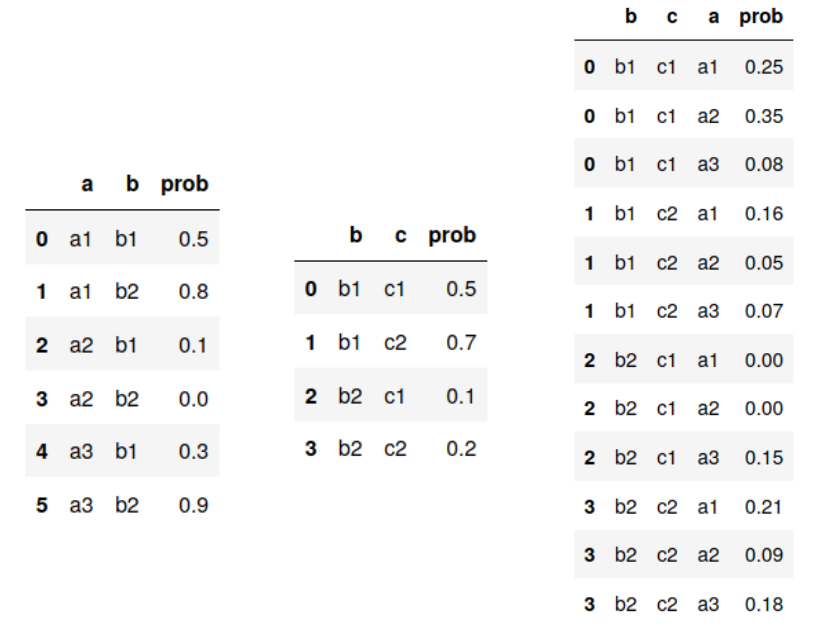
\includegraphics[width=.4\textwidth]{img/table.png}
    \caption{Caption here.}
    \label{fig:exampleFig}
\end{figure}

Referencing a figure in text is done with its label and the ref command like so, Figure \ref{fig:exampleFig}.\\

To create a table we use the table command. To change the amount of columns you alter the parameter after tabular. For more styling I refer to the Overleaf table \href{https://www.overleaf.com/learn/latex/Tables}{\bf{documentation}}.
\begin{table}[H]
    \centering
    \begin{tabular}{c  c  c}
        column name 1 & column name 2 & column name 3 \\ [0.5ex]
        \hline\hline
        1 & 389.27 & 249.95 \\ [1ex]
        
        2 & 310.20 & 197.19 \\ [1ex] 
        
        3 & 563.48 & 322.50 \\ [1ex] 
        
        4 & 550.58 & 308.64 \\ [1ex] 
        
        5 & 415.76 & 248.32 \\ [1ex] 
        \hline
    \end{tabular}
    \caption{Caption here.}
    \label{table:errorsTable}
\end{table}

\newpage

For multiple images in one figure we use subfigures. The double forward slash splits up the line of images, removing it results in the images being aligned horizontally.
    \begin{figure}[H]
    \centering
    \subfloat[Sub Image 1]{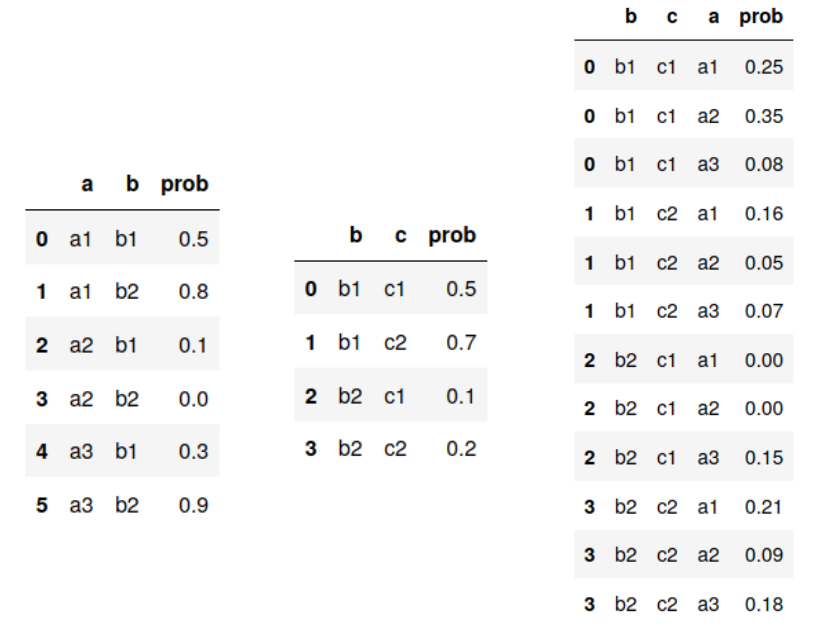
\includegraphics[width=.3\textwidth]{img/table.png}}
    \subfloat[Sub Image 2]{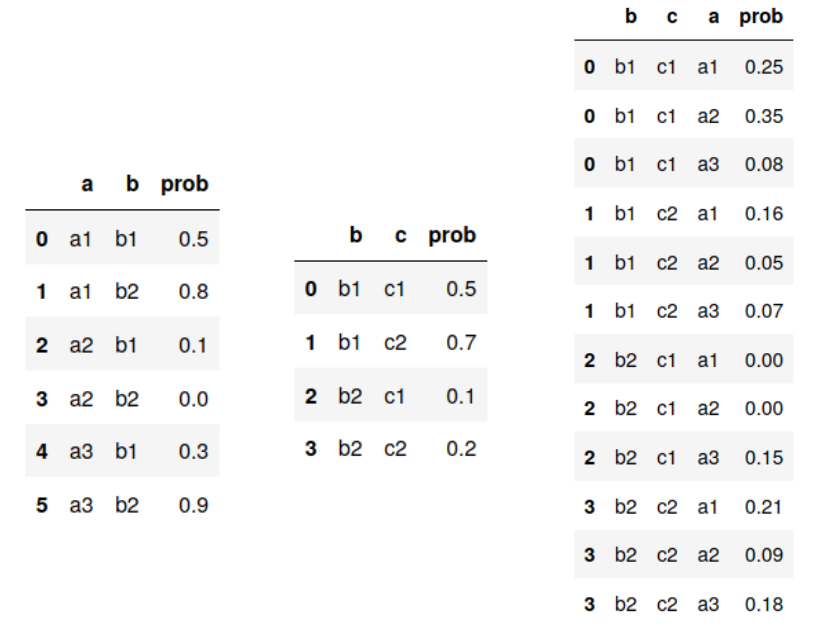
\includegraphics[width=.3\textwidth]{img/table.png}}\\
    \subfloat[Sub Image 3]{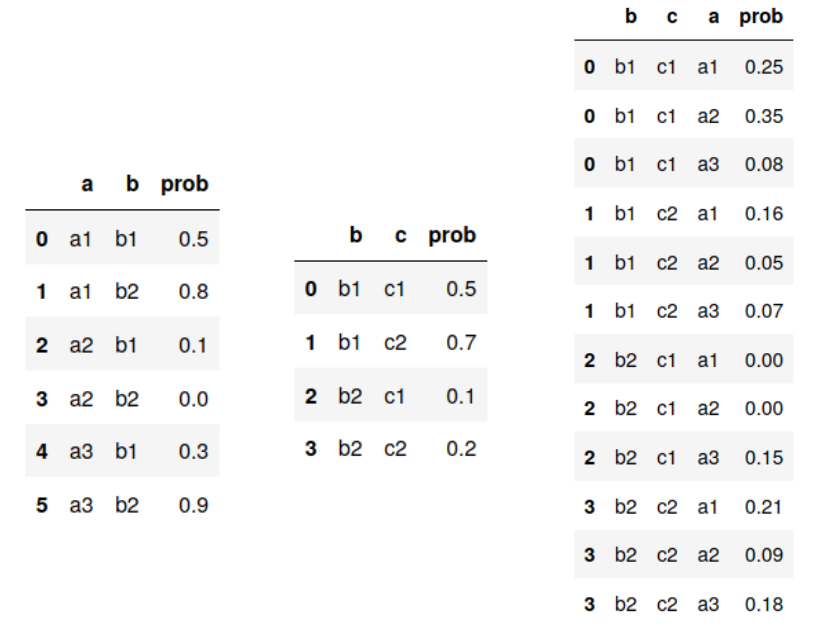
\includegraphics[width=.3\textwidth]{img/table.png}}
    \subfloat[Sub Image 4]{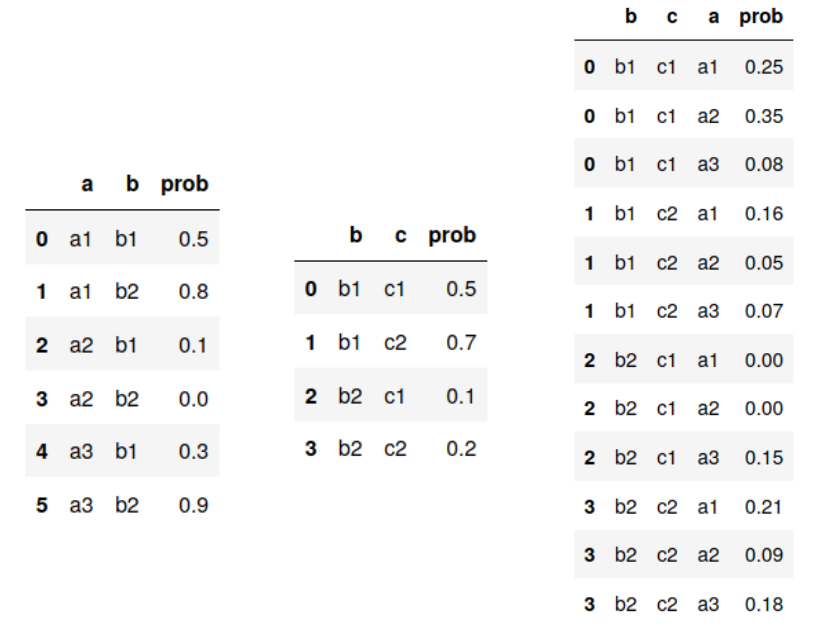
\includegraphics[width=.3\textwidth]{img/table.png}}
    \caption{Caption here.}
    \label{fig:examplesSubFig}
\end{figure}

\end{document}